\documentclass[a4paper]{article}

%% Language and font encodings
\usepackage[english]{babel}
\usepackage[utf8x]{inputenc}
\usepackage[T1]{fontenc}

%% Sets page size and margins
\usepackage[a4paper,top=2.5cm,bottom=2.5cm,left=2.5cm,right=2.5cm,marginparwidth=1.75cm]{geometry}

%% Useful packages
\usepackage{amsmath}
\usepackage{graphicx}
\usepackage[colorinlistoftodos]{todonotes}
\usepackage[colorlinks=true, allcolors=blue]{hyperref}
\usepackage{subfigure}
\usepackage{caption}
\usepackage{amsfonts}
\usepackage{amsthm}
\usepackage{upquote}
\usepackage{listings}
\usepackage{enumitem}
\usepackage{dirtytalk}
\usepackage{hyperref}
\usepackage{float}

\usepackage{xcolor}
\usepackage{indentfirst}

\linespread{1.1}

\definecolor{mGreen}{rgb}{0,0.6,0}
\definecolor{mGray}{rgb}{0.5,0.5,0.5}
\definecolor{mPurple}{rgb}{0.58,0,0.82}
\definecolor{backgroundColour}{rgb}{0.95,0.95,0.92}
\lstdefinestyle{CStyle}{
    backgroundcolor=\color{backgroundColour},
    commentstyle=\color{mGreen},
    keywordstyle=\color{magenta},
    numberstyle=\tiny\color{mGray},
    stringstyle=\color{mPurple},
    basicstyle=\footnotesize,
    breakatwhitespace=false,
    breaklines=true,
    captionpos=b,
    keepspaces=true,
    numbers=left,
    numbersep=5pt,
    showspaces=false,
    showstringspaces=false,
    showtabs=false,
    tabsize=2,
    language=C
}


\def\therefore{\boldsymbol{\text{ }
\leavevmode
\lower0.4ex\hbox{$\cdot$}
\kern-.5em\raise0.7ex\hbox{$\cdot$}
\kern-0.55em\lower0.4ex\hbox{$\cdot$}
\thinspace\text{ }}}

\title{A Journey to the Interactive 3D Fractal World}
\author{CSED Yang Junha 20160785, Ryu Sangwoo 20160845, Sung Haebin 20160463}

\begin{document}
\maketitle
\begin{abstract}
We researched and developed a program that presents interactive 3D fractal world in real time.
Our main idea is to seperate pixel-level fractal and polygonal fractal and combine them with texture.
To do this in an interactive way, the fractals should be rendered dynamically and efficiently.
We designed our own rendering pipeline and present some ideas to achieve interesting features of factal rendering.
And finally we've succeeded on implementing actual program with OpenGL.
\end{abstract}
\section{Motivation}
Fractals are so beautiful.
Their structures are so delicate and impressive, with a very simple underlying mathematical principle.
Just watching fractal growing is enough to bring inner peace in your mind.
For example in Youtube, tons of videos that just render fractals earn million views.

We thought that developing a realtime interactive 3D fractal renderer would be awesome,
because it'll be fun to design our own fractal, and meaningful to share our experience of fractals to others.
This program is definetly not a game, nor a solution to a certain mathematical problem.
We'll just say that our project is a `visual experience' of the fractals.
It would be for fun, for education, for some artistic production, or even for Youtube!

Another aim of this project is to practice various concepts covered in lecture and get more skillful in computer graphics.
We've tried adopt basic principles of computer graphics as many as possible(OpenGL, shaders, shading, modeling, deformation, texture, hierarchy, antialiasing, animation..)

\section{Theoretical Backgrounds}
\subsection{Fractal}
A fractal is a recursive, infinitely self-reproductive geometric pattern.
Fractals have similar patterns at smaller scales.
So if we zoom into a fractal, we could experience a delicate, complex, repetitive, and varying pattern.
A fractal is usually defined as a mathematical recursive equation.
There are some known techniques of generating a fractal;
The types that we used are Escape-time fractals and Finite subdivision rules.
Escape time fractals use a formula at each point in a space to determine the pattern.
Finite subdivision rules use a recursive topological algorithm to define the pattern.
We use the terms \textit{pixel level fractal} for the escape time fractal, and \textit{geometric polygonal fractal} for the finite subdivision rule in this report.
\subsection{Mandelbrot Set}
The mandelbrot set is an example of escape time fractals.
It is defined as whether a function $f_c(z) = z^2 + c$ diverges or not if the point is $c$ in a complex plane, while the function is iterated from $z = 0$.
If it the value remains bounded, then it is part of a mandelbrot set.
It is hard to check if it diverges or not in reality, so we just take an approximative method; iterate the function for a certain number of loops, and check if it has an L2-norm value bigger than 2.
But this iteration causes some bottleneck if the iteration count gets higher, so we have a limitation on the complexity of the Mandelbrot.
The definition of mandelbrot set is just a set with only binary information, so we often make use of additional metrics to gather some additional visual information.
\begin{figure}[H]
\centering
\subfigure[Mandelbrot set]
{
    \label{fig:subfig1}
    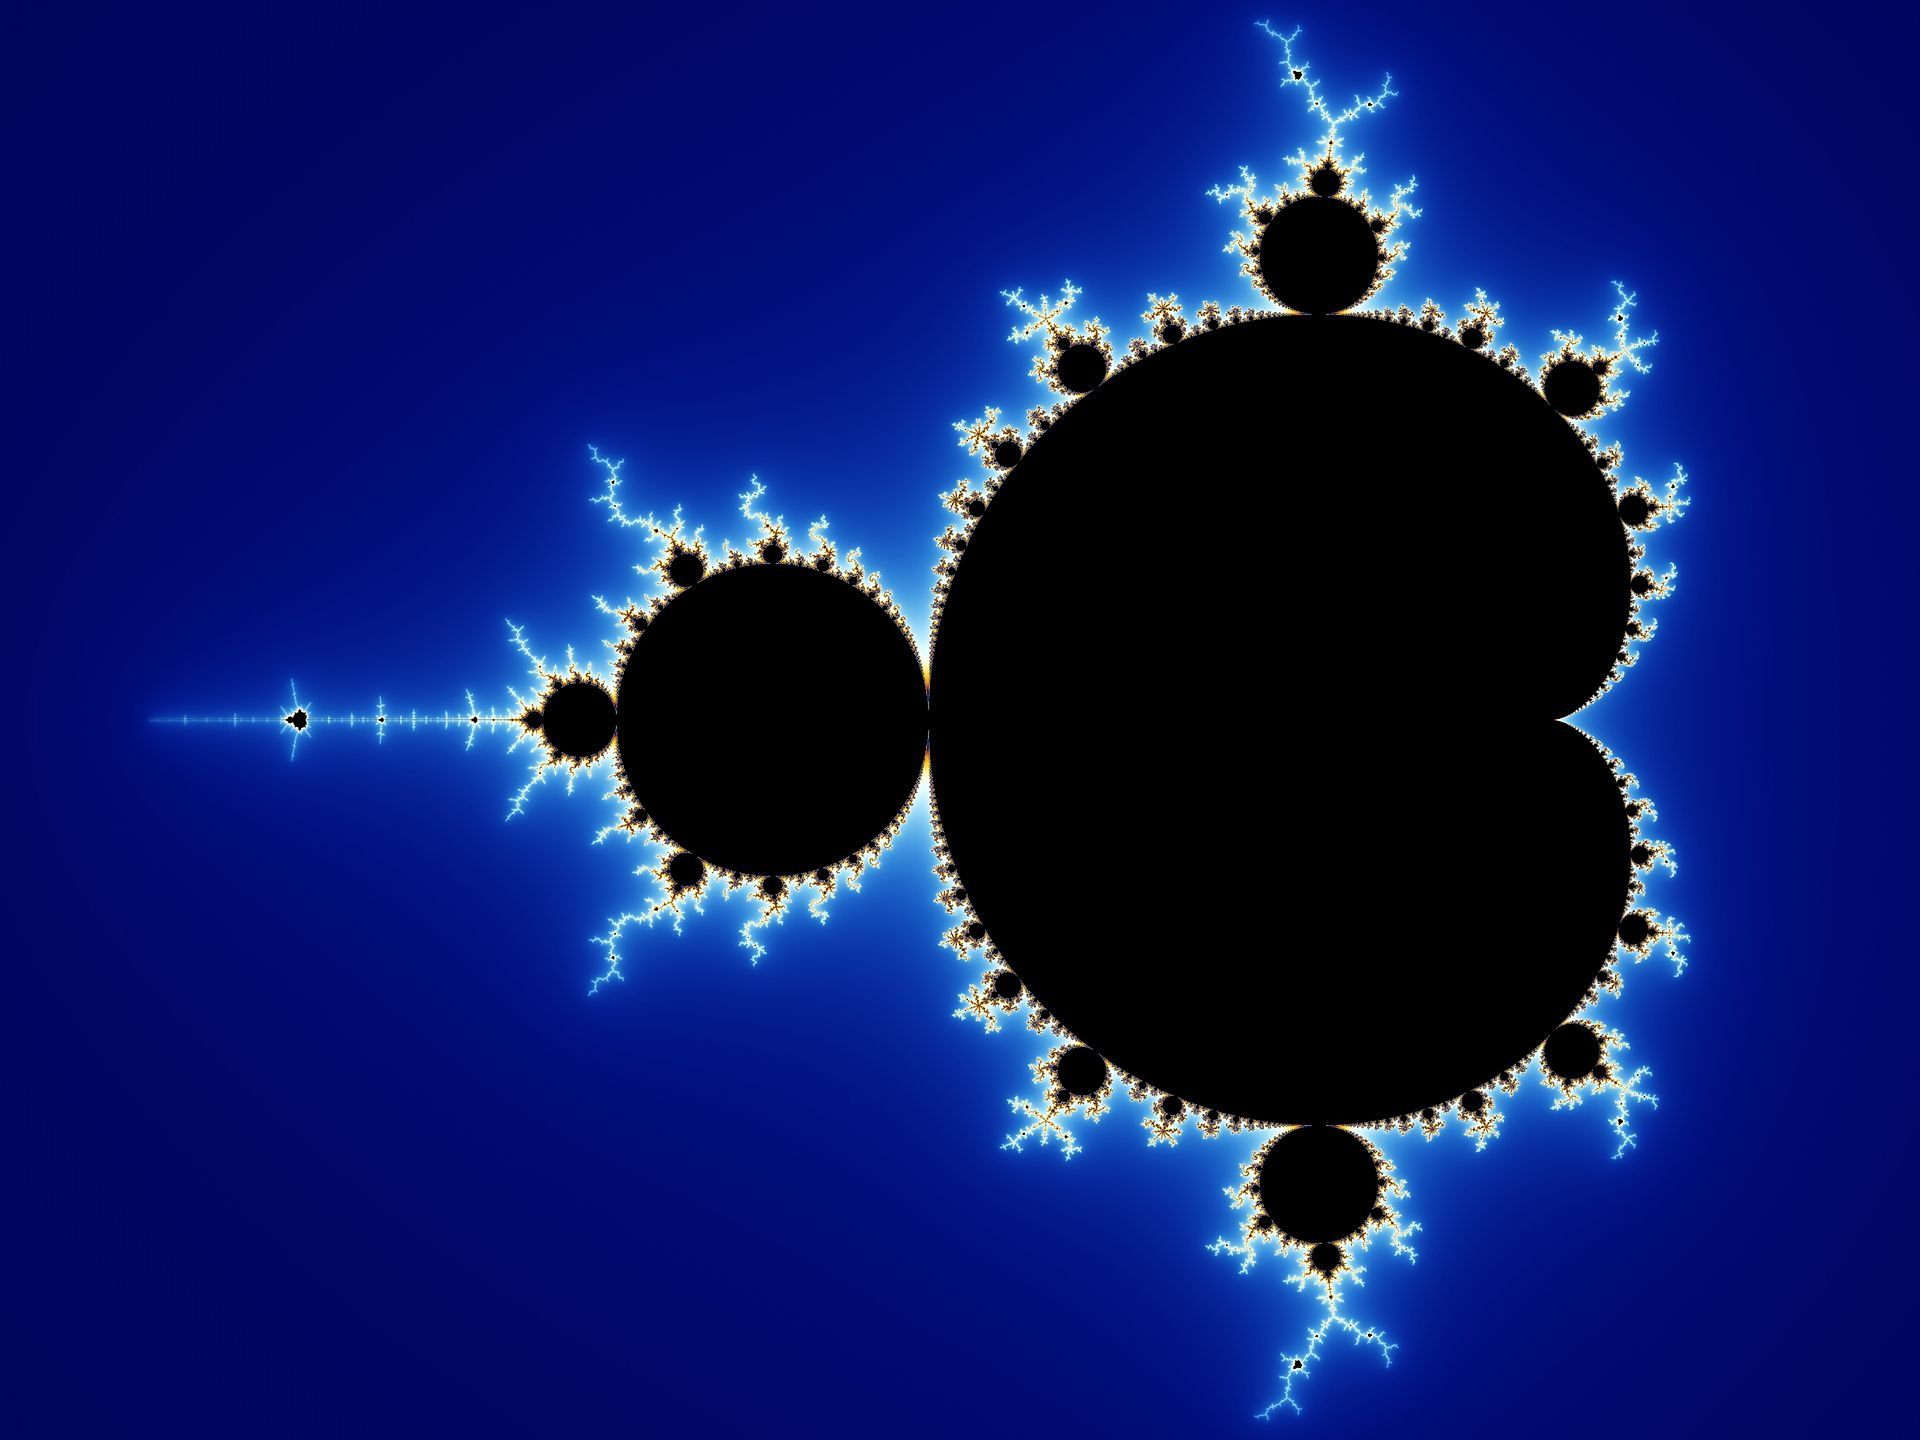
\includegraphics[scale=0.3]{mandel.jpg}
}
\end{figure}

\section{Task}
Again, we're goal is to implement a program that present real-time rendering of 3D fractal world with interaction.
There are some fractals which are pixel-level but also in 3D space.
One of example is `Mandelbulb', which is kind of generalization of Mandelbrot set onto 3D coordinates.
That kind of fractals of course can yield beautiful 3D fractal world, however very exepensive because it is basically voxel calculation.

Instead, we take our approach as `fractal on fractal'.
That means \textbf{Mandelbrot set, the pixel level fractal is textured on 3D geometric polygonal fractal}.
By doing this, we can get nice 3D fractal world with relatively reasonable cost.
To give impression of `wandering in the fractal world', the camera will stay \textit{inside} the geometric fractal, whereas the Mandelbrot set is covered on that.
There are many issues with doing this, and we solve them one by one with our own ideas. (will be explained in \ref{sec:2})
Our goal is to design well-structured rendering pipeline and to implement all required process into real executable program.


\section{Ideas and Implmentation}\label{sec:2}
\subsection{Development Environment and Codes}
We develop everything in C++ and OpenGL only.
As we mentioned in proposal, utilizing shaders directly is essential for what we do.
Thus we chose OpenGL for our development environment.

If you want to know about details about our codes,
we recommend you to read Assignment 2-4 report of Yang and Sung, because we adopt basic OpenGL structure from those.
Here are some notable source codes.
\begin{itemize}
  \item void CGraphics::M\_SimplePolyFractal(void) constructs hierarchy for fractal.
  \item void CGraphics::M\_RenderFractal(void) renders fractal.
  \item bool CGraphics::M\_MoveRequest(Vec3d d) takes movement info and expands. (see \ref{sssec:num1}.)
  \item `ver\_shd.glsl' and `frag\_test.glsl' are shaders for fractal.
\end{itemize}
\subsection{Rendering a Mandelbrot set}
As stated in the above, the mandelbrot set itself is just binary classification; whether it is in the mandelbrot set or not.
For better visualization rather than two colors, we gather some information derived from the mandelbrot iteration.
The first information we gathered is the amount of iterations when the non-mandelbrot set point has diverged (got bigger than our threshold).
The second information is the ratio of real value and imaginative value of $f_c(z)$ when the iteration ended.
Using these metrics, we generated a colorful and beautiful visualization of Mandebrot set.
We also chose an adequate coordinate to zoom up the fractal, and this constant zooming up and down is the final texture we are going to use in the 3d polygon fractal.
When we zoomed the fractal, we did not manipulate the camera position in OpenGL, because we needed to integrate this mandelbrot into texture of the polygon fractal.
Instead, we used a zooming mechanism solely in the shader, an that is what we call camera seperation (geometric and pixel).
\begin{lstlisting}[style=CStyle]
//fragment shader code

//mandelbrot set iteration
int i;
for(i = 0; i < max_iter; i++)
{
  double nx = x*x-y*y + c.x;
  double ny = 2*x*y + c.y;

  if (nx*nx + ny * ny > max)
    break;

  x = nx;
  y = ny;
}

//additional metrics for visualization
float a = float(i) / (max_iter);
float b = tanhnorm(float(x/(y)));

//combine metrics with texture to create pattern
vec2 uv;
uv.x = sinnorm(exp(exp(a)) * b);
uv.y = sinnorm(exp(exp(b)) * a);
vec4 color1 = texture2D(pallete, uv) * (1 - a) * a * b;

uv.x = sinnorm(exp(exp(a)));
uv.y = sinnorm(exp(exp(a)));
vec4 color2 = texture2D(pallete, uv) * (1 - a) * a;


vec4 clr = color1 * 2  +  color2 * 2.5;
clr[3] = 1;
color = clr;
\end{lstlisting}
\begin{figure}[H]
\centering
\subfigure[Texture Pallete for Mandelbrot Visualization]
{
    \label{fig:subfig1}
    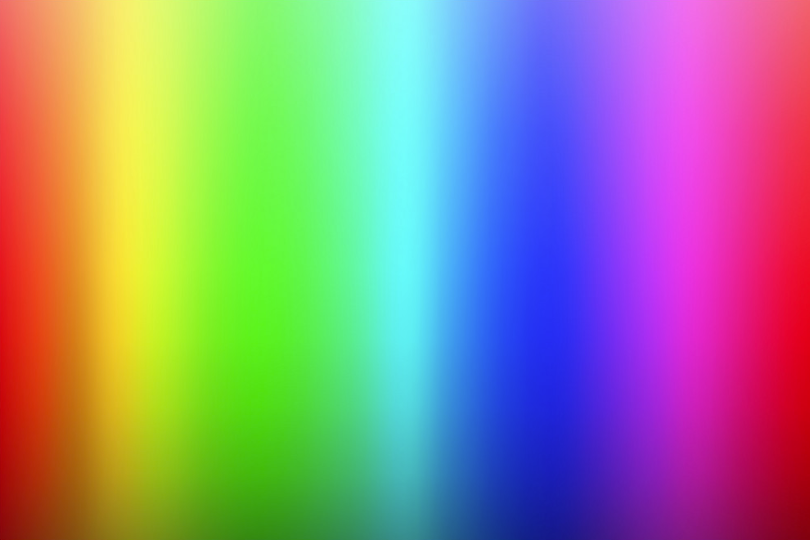
\includegraphics[scale=0.3]{pallete.png}
}
\subfigure[Result of Mandelbrot Visualization]
{
    \label{fig:subfig1}
    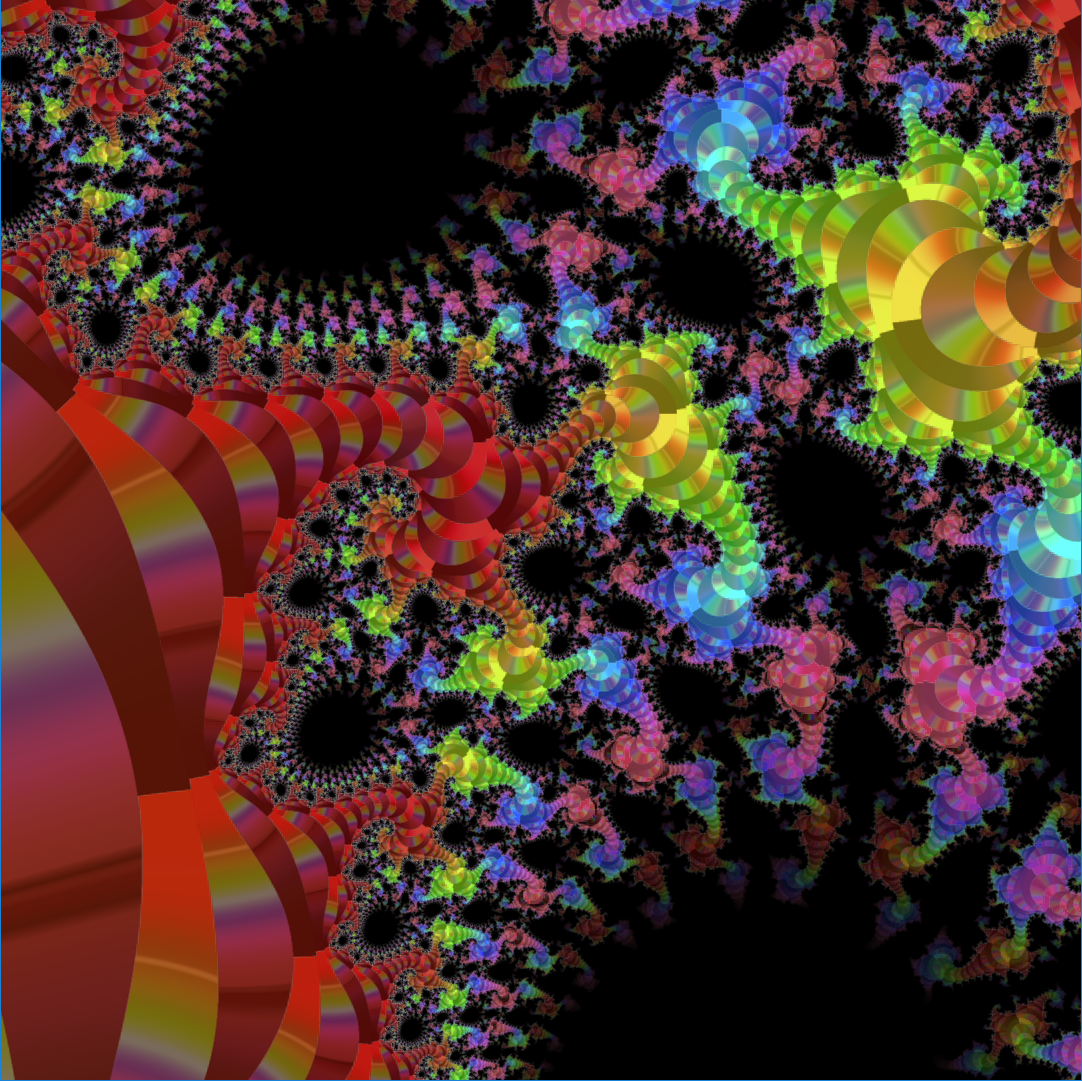
\includegraphics[scale=0.5]{beauty.png}
}
\end{figure}

\subsection{3D Geometric Fractals}
\subsubsection{Meshes}
We have two basic meshs to implement geometric fractals.
One is sphere with 6 holes, another is wormhole to connect between spheres
Because we have to connect to meshes smoothly, we construct wormhole with splines covering sphere using Loft NURBS in MAXON Cinema 4D, and apply subdivision surface.
Mesh with one sphere and one wormhole is one node in hierachical structure, and basic unit of expansion.
\begin{figure}[H]
\centering
\subfigure[Sphere with 6 holes]
{
    \label{fig:subfig1}
    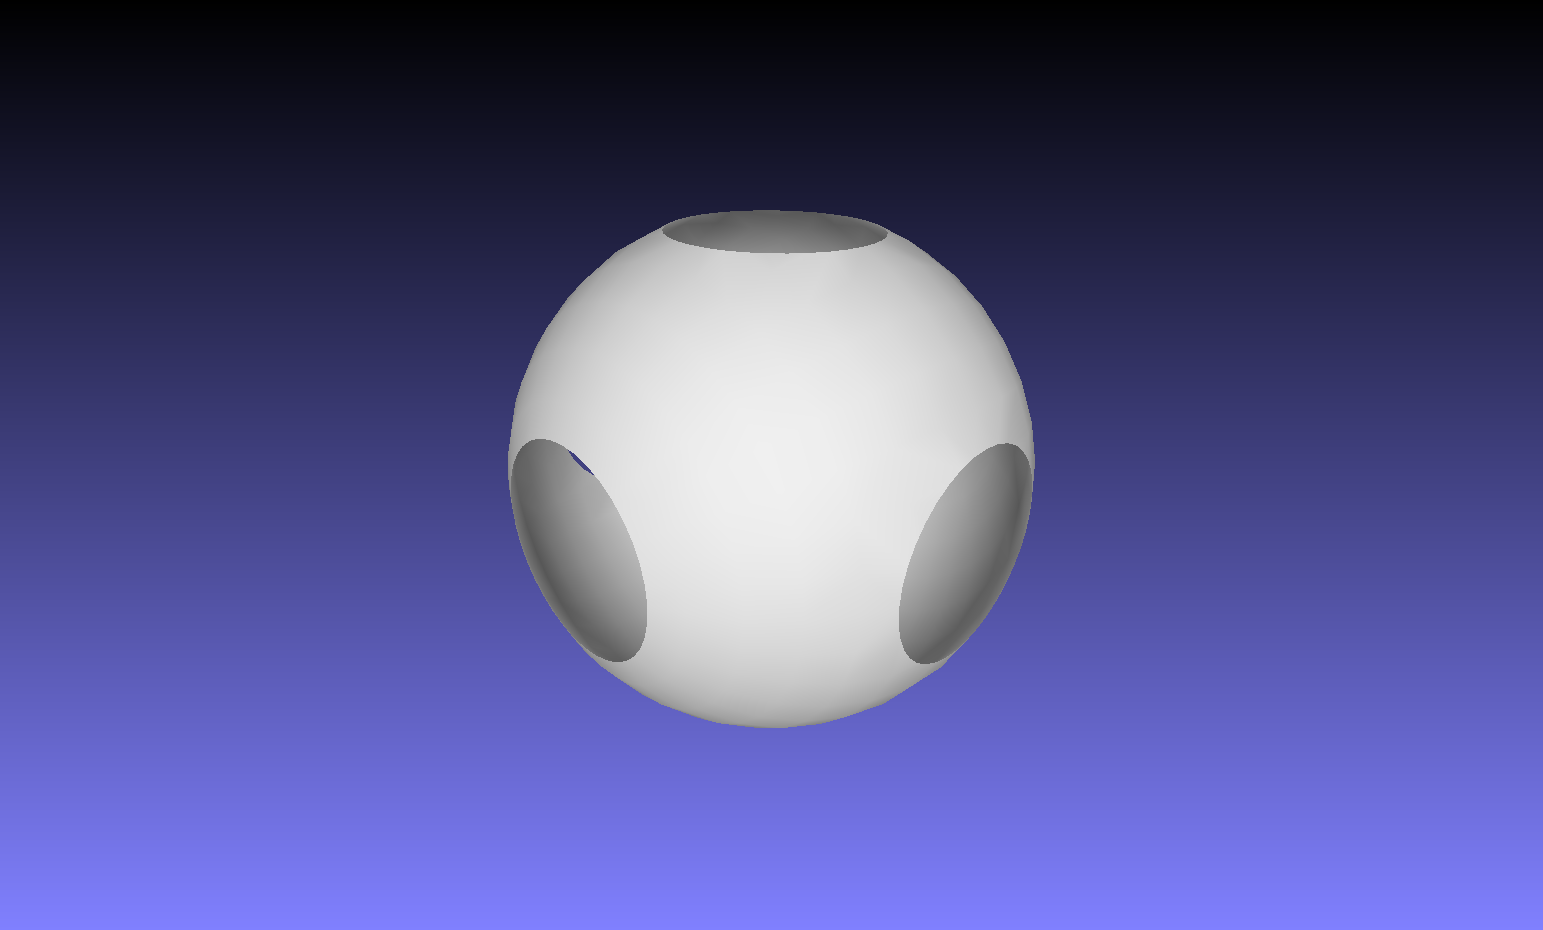
\includegraphics[scale=0.1]{sphere.png}
}
\subfigure[Wormhole]
{
    \label{fig:subfig1}
    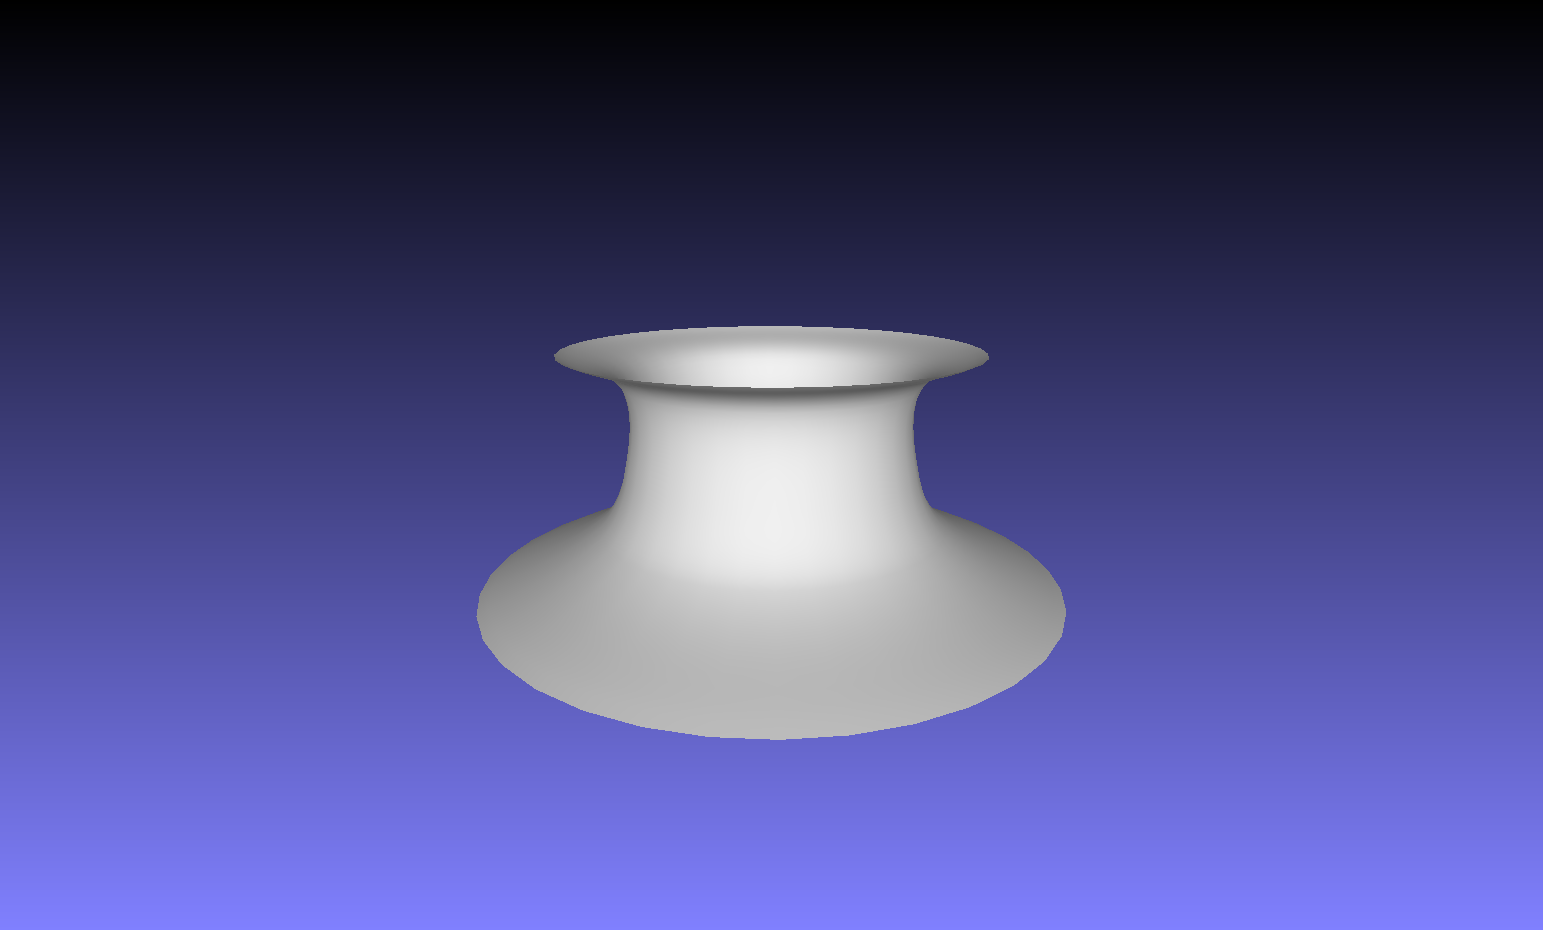
\includegraphics[scale=0.1]{wormhole.png}
}
\caption[1]{Hierarchical model for fractal.}
\end{figure}

\subsubsection{Hiearchy}
Geometric fractals can be regarded as a special case of hierarchical model.
But, the hierarchical transfomrations are given \textit{recursively}, and each nodes have same rendering function.
If we give two recursive hierarchical transfomrations, then the fractal will grow double for each step, because the tree will be branched twice.
Then specify the maximum depth, and we can get a nice geometric fractal.
In this project, we construct the geometric fractal with 5 recursive transformation.
\begin{figure}[H]
\centering
\subfigure[5 direction of recursive transformations]
{
    \label{fig:subfig1}
    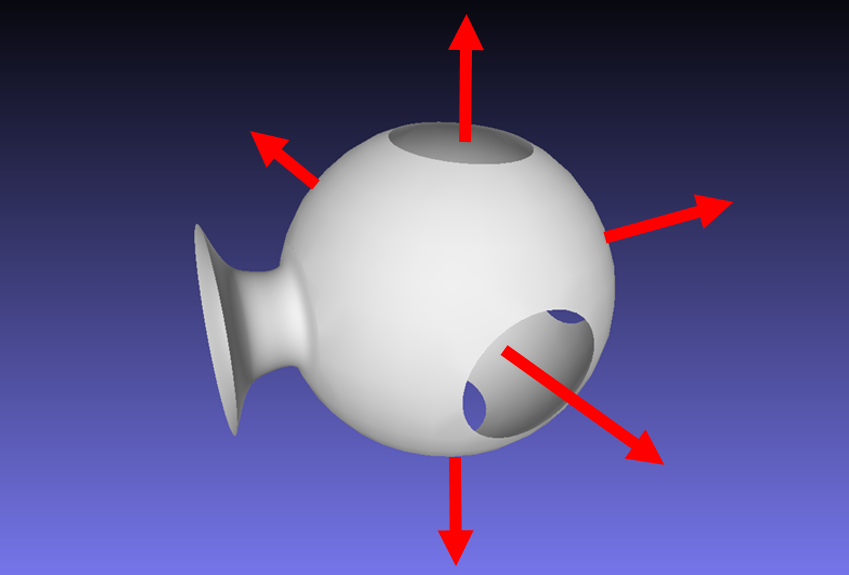
\includegraphics[scale=0.2]{hier.PNG}
}
\subfigure[Exapnded in maximum steps of 2]
{
    \label{fig:subfig1}
    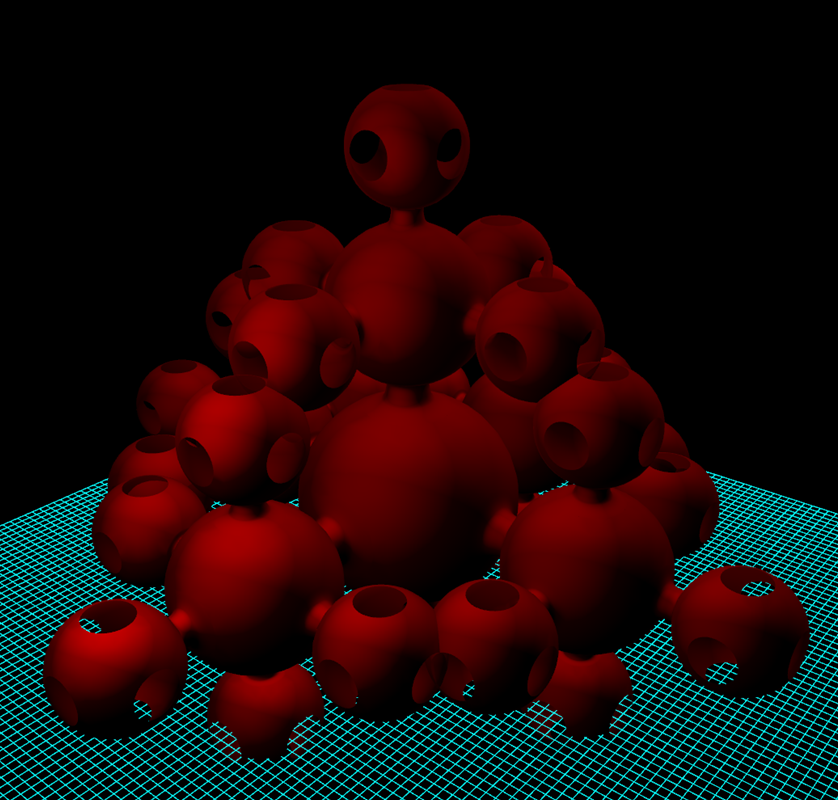
\includegraphics[scale=0.2]{expand.PNG}
}
\caption[1]{Hierarchical model for fractal.}
\end{figure}

\subsubsection{Path Tracking}\label{sssec:num1}
To `wander' into the fractal world, that geometric fractal should be somewhat `surrounding' environment for viewer.
That means the camera will move \textit{inside} the fractal, and the should able to explore deeply.
This going-through must be availiable infinitely, and this is a problem.

If we simply expand fractal in more depth, the program will die soon. (remember that the nodes grow exponentially.)
Even 10 steps require $5^{10}=9,765,6254$ nodes in the scene.
Thus we should render only relevant nodes according to current position of camera.
The idea here is to keep track of recursion path of current node.

\begin{figure}[H]
\centering
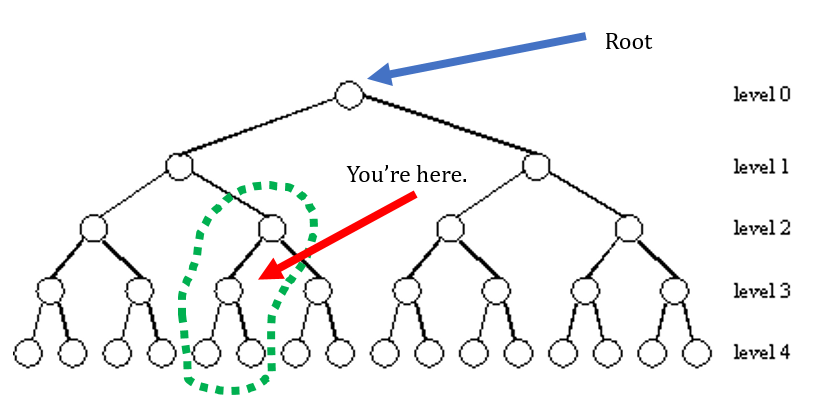
\includegraphics[scale=0.5]{tree.png}
\caption[q]{Recursive hierarchy tree. Note that the branches are reduced in 2 steps for simplicity.}
\label{fig:tree}
\end{figure}

If the program keep track of the path which the camera had moved along, then we know exactly where we are in big tree of hierarchy.
Then, the rendering pipeline can choose \textit{relevant} nodes to camera, and can partially render them.
For example, in figure \ref{fig:tree}, those nodes in the green line will be chosen to be rendered.

To track the path(or trace), we should check every single movement of camera.
If the camera goes outside of current node, then see the direction(one of 5) and push it on path stack.
\begin{enumerate}
  \item Accumulate all recursive transformation using the path.
  \item Get the transformation M.
  \item Take inverse of M and multiply on my position to take everything into node(model) space.
  \item Perform a collision detection for each 6 sides of node.
  \item Find out the branch of recursion and stack on my path.
\end{enumerate}

\begin{figure}[H]
\centering
\subfigure[Partial rendering by path tracking. Note that this viewing is from another camera, and real camera is now inside the polygon.]
{
    \label{fig:subfig1}
    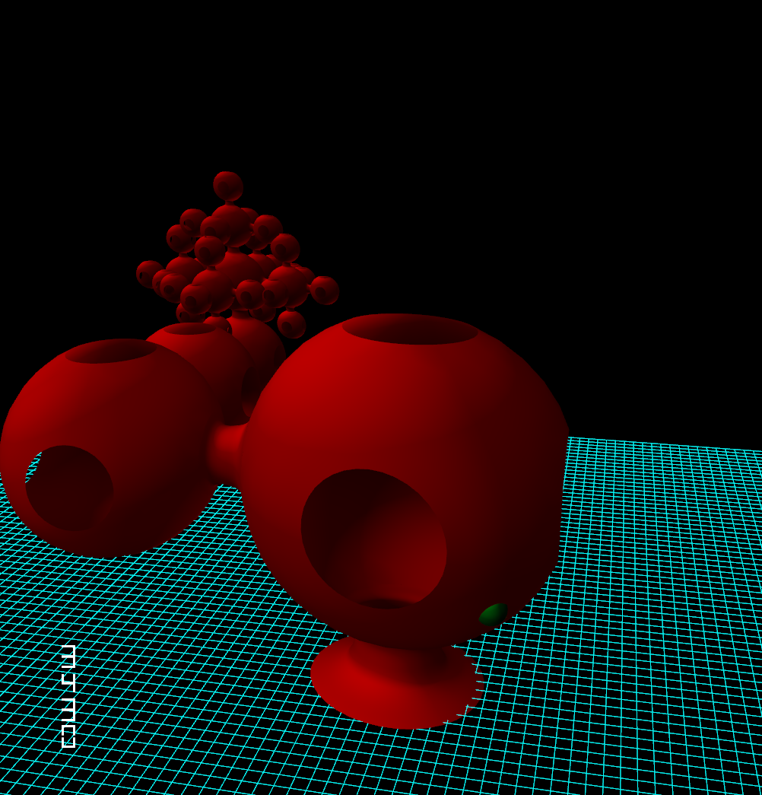
\includegraphics[scale=0.5]{path1.PNG}
}
\subfigure[From another view.]
{
    \label{fig:subfig1}
    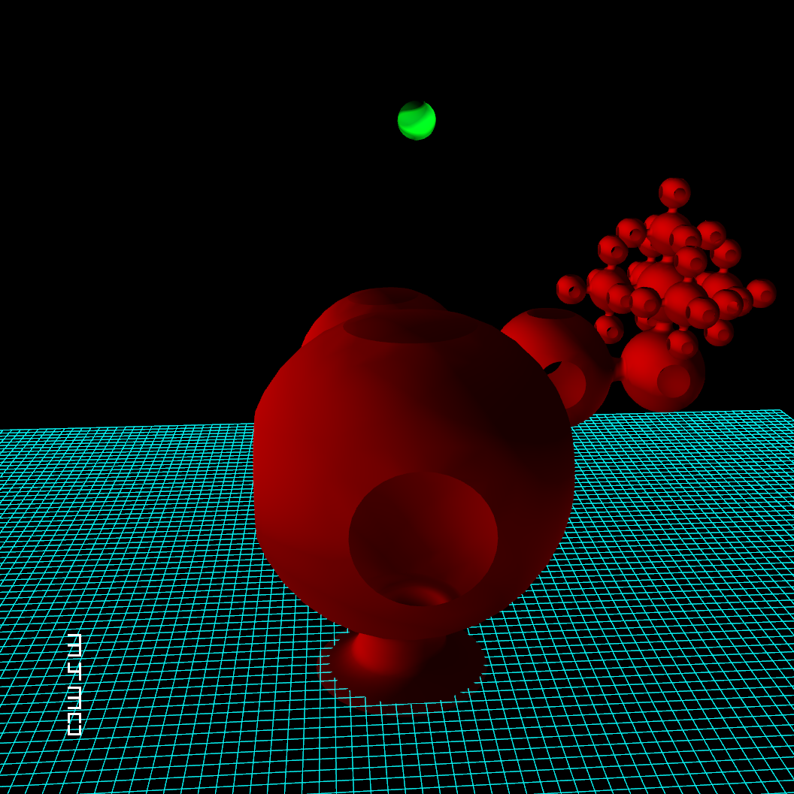
\includegraphics[scale=0.5]{path2.PNG}
}
\caption[1]{Path tracking is now on.}
\end{figure}

\subsection{Texture Mapping}
Now we have to combine those seemingly independent two fractals (Mandelbrot and geometric).
Again, our approach is `fractal on fractal' and key idea is take Mandelbrot set as a `texture' for the polygons, the geometric fractal.
The texture coordinate from polygon will be used as coordinate in Mandelbrot set,
Note that the program keep two camera, one for Mandelbrot set and one for 3D world(with geometric fractal).
Then it will be like that Mandelbrot set is traversed with some movement, while being projected on fractalistic polygons.

We tried to assign pre-determined texture coordinates on mesh itself,
but it was very difficult to match continuity between wormhole and sphere. (Remeber there are 8 holes and all should be synchronized)
Instead, we just dynamically assign texture coordinate via simple mathematical formulation.

For this, two things musd be considered very carefully.
\begin{itemize}
  \item Texture coordinates should be continuous everwhere.
  \item Mandelbrot set lies on limited space, somewhere around (-1, 1).
\end{itemize}

Keeping texture coordinate continous can be achieved by using vertices' world coordinate, because they are also continous in world.
Of course the 3D coordinates should be transformed into 2D one, so we combined them linearly.
And for the domain (-1, 1), we just take sin of cooridnates.

\begin{align*}
T_x&=sin(F(P_x+P_y))\\
T_y&=sin(F(P_y+P_z))
\end{align*}
Here $T$ is texture coordinate, $P$ is world coordinate, and $F$ is coefficient about fractal scale.
\subsection{Shading}
Shading is important for viewer to percept spatial structure even in non realistic fractal world.
It could be confusing to wander 6-sided chambers freely in 3D dimension.
So we applied basic shading (diffuse, specular ...) on polygons.
Assignment4 was helpful for this.

\subsection{Deformations}
We apply realtime deformation on geometric fractal, to get some interesting spatial effect.
We can easily impose some distortion on vertices in vertex shader, with time variable $t$ and sin.
The problem is keeping both C0 continuity and C1 continuity on the sphere and wormhole.
That's because we always put them together but they are separated meshes in program, for further flexible reconstruction of geometry.
C0 continuity is easy because it's not a problem if we can apply same transformation on joint.

C1 continuity, or smoothness is hard to achieve, so we just rather make `illusion' of smoothness.
The idea is \textit{not} transforming normal vectors together.
Since we already created the meshes with smooth normal vectors, if we transform only positions, then the smoothness via shading will be preserved.

\begin{figure}[H]
\centering
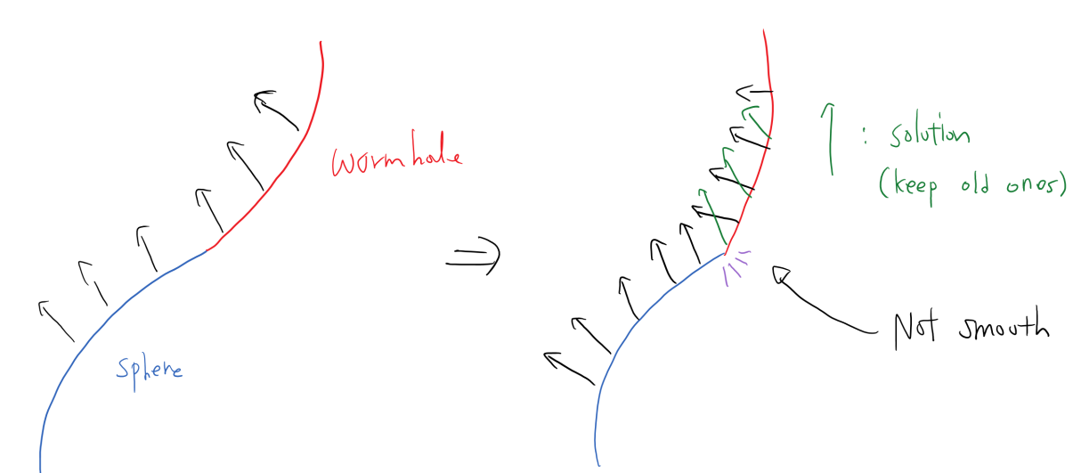
\includegraphics[scale=0.5]{smooth.png}
\caption[q]{If we take green arrows (not transformed normal vectors) the normals are smooth although actual curve is not smooth.}
\label{fig:tree}
\end{figure}

\subsection{Camera control}
We have two methods moving camera.
One is with keyborad input, another is with mouse moving.
When we give keyboard input, camera moves to 6 direction without rotation. (wasd, space bar and shift)
When we give mouse moving, camera rotates.
These are very basic camera movement, so we want more cinematic movement.
Basic camera model gives us jerky movement, that is, it responses immediately and honestly like normal FPS game when we give input.
But we want more smooth movement, we introduced momentum and time variation to movement.
\begin{itemize}
  \item void CGraphics::M\_MoveCamera(void) moves camera with smooth motion.
\end{itemize}
In case of keyboard, we just give acceleration when camera starts and stops moving.
In case of mouse, we interpolated mouse position with logarithmic term that depends on time.

\subsection{Antialiasing}
Antialiasing is one of the important process in high-quality rendering.
For the geometric fractal, only multi-sampling is ok because it consists of just polygons.
However the textured Mandelbrot set can't be antialiased in that way because it shows very complex structrue in \textit{pixel level}.
Of course all pixel-level rendering doesn't have to be antialiased.
For example, antialiasing the shading won't that helpful because it is inherently smooth.
But Mandelbrot set is very complicatedly structured and the pixels vary greatly, so antialisaing maybe essential.

Unfortunately, we concluded that the only way to perform antialiasing is by super-sampling because there's no way to infer something, but only calculating multiple times.
Thus we tried to perform antialiasing in fragment shader by doing Mandelbrot set membership test multiple times.
We varies testing coordinates slightly within an one pixel size for each sampling, and blend them for final output.

\begin{figure}[H]
\centering
\subfigure[Mandelbrot set without antialiasing]
{
    \label{fig:subfig1}
    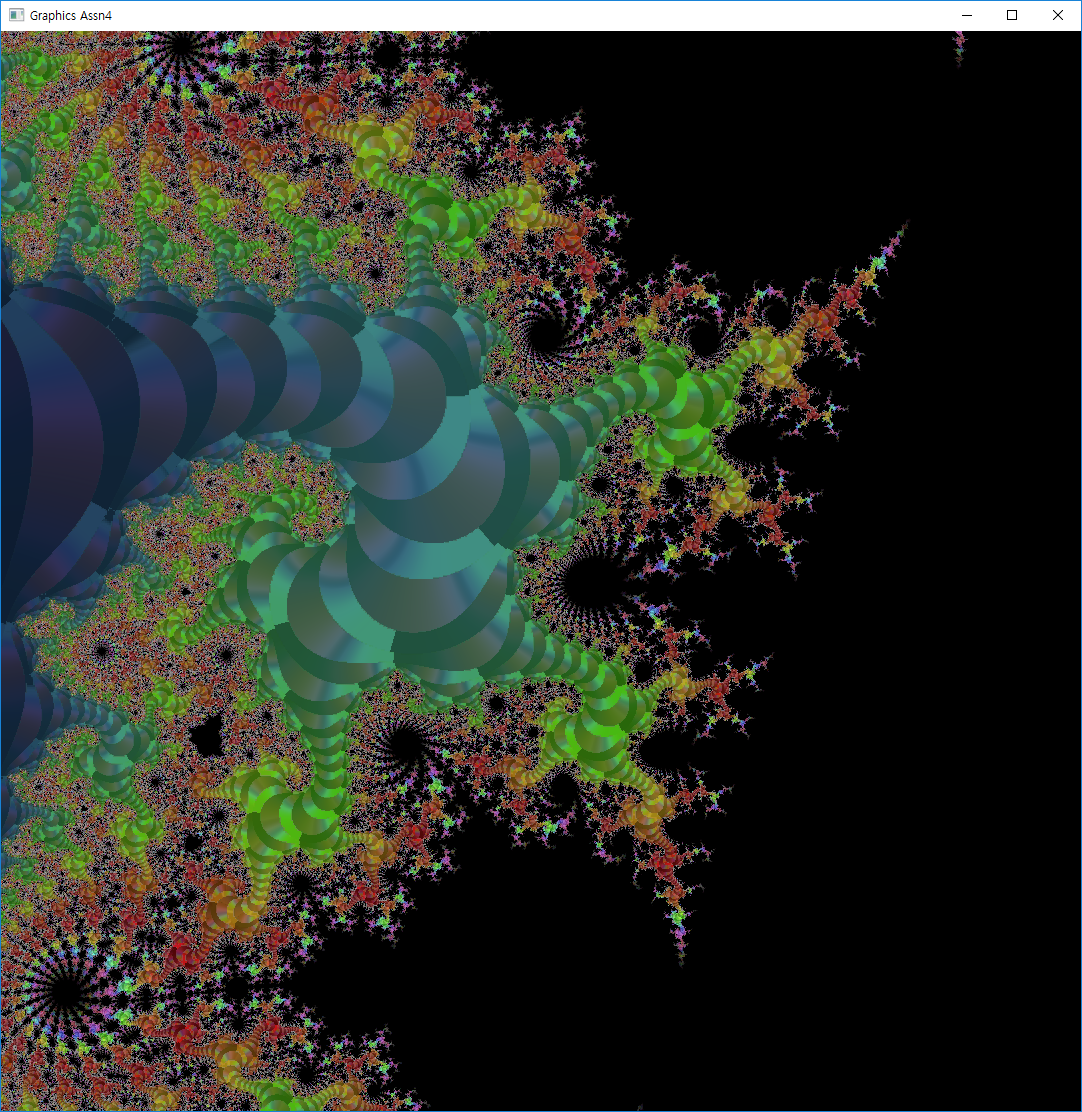
\includegraphics[scale=0.2]{noanti.PNG}
}
\subfigure[Mandelbrot set with antialiasing]
{
    \label{fig:subfig1}
    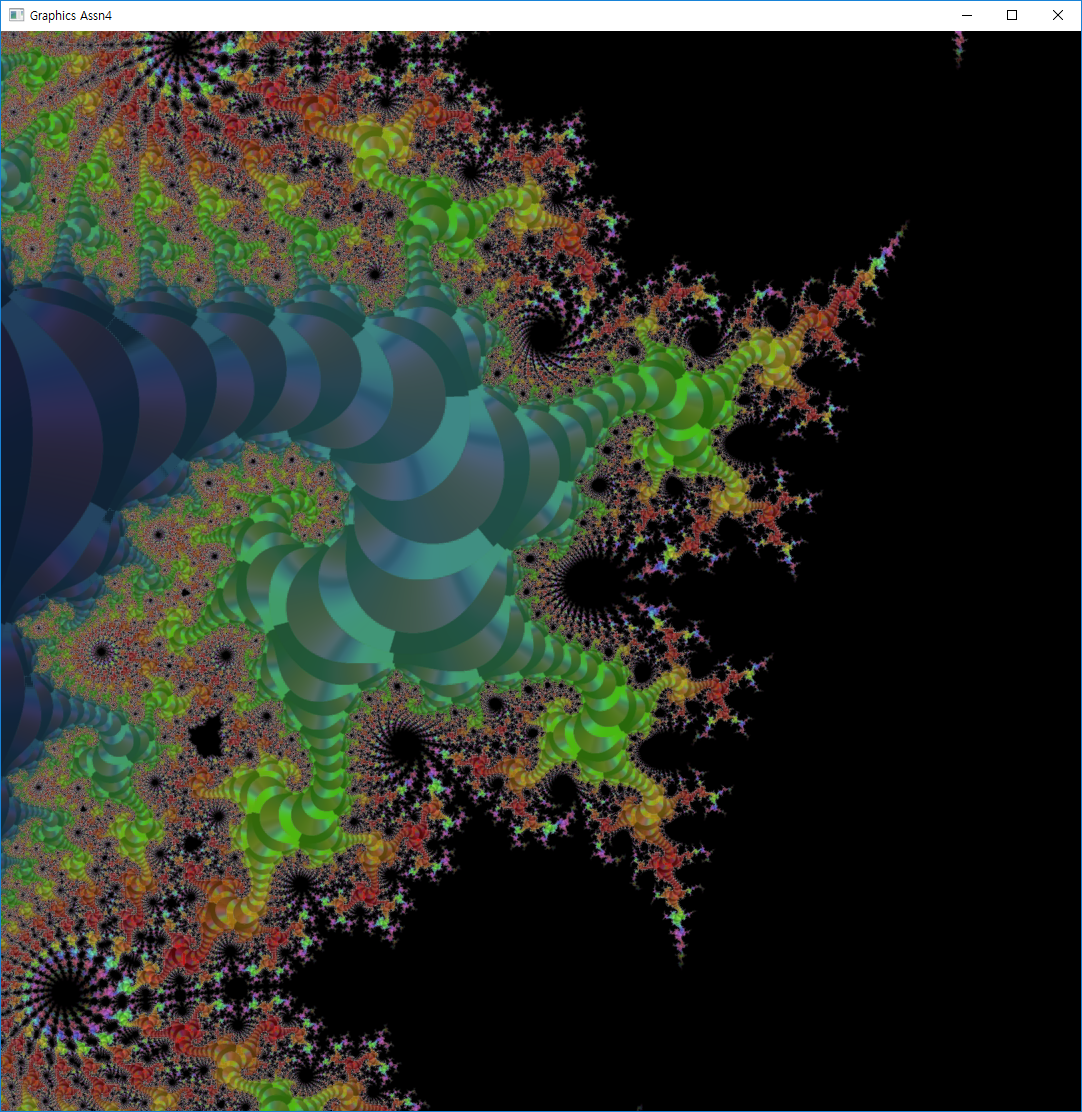
\includegraphics[scale=0.2]{anti.PNG}
}
\caption[1]{Antialiasing comparison}
\end{figure}
We found that rendering quality has been improved but the rendering cost gets very expensive. (fps becomes $<20$)
One of our goal for this project is `real time', so we just discard the antialising.

\section{Gallery}
\begin{figure}[H]
\centering
\subfigure
{
    \label{fig:subfig1}
    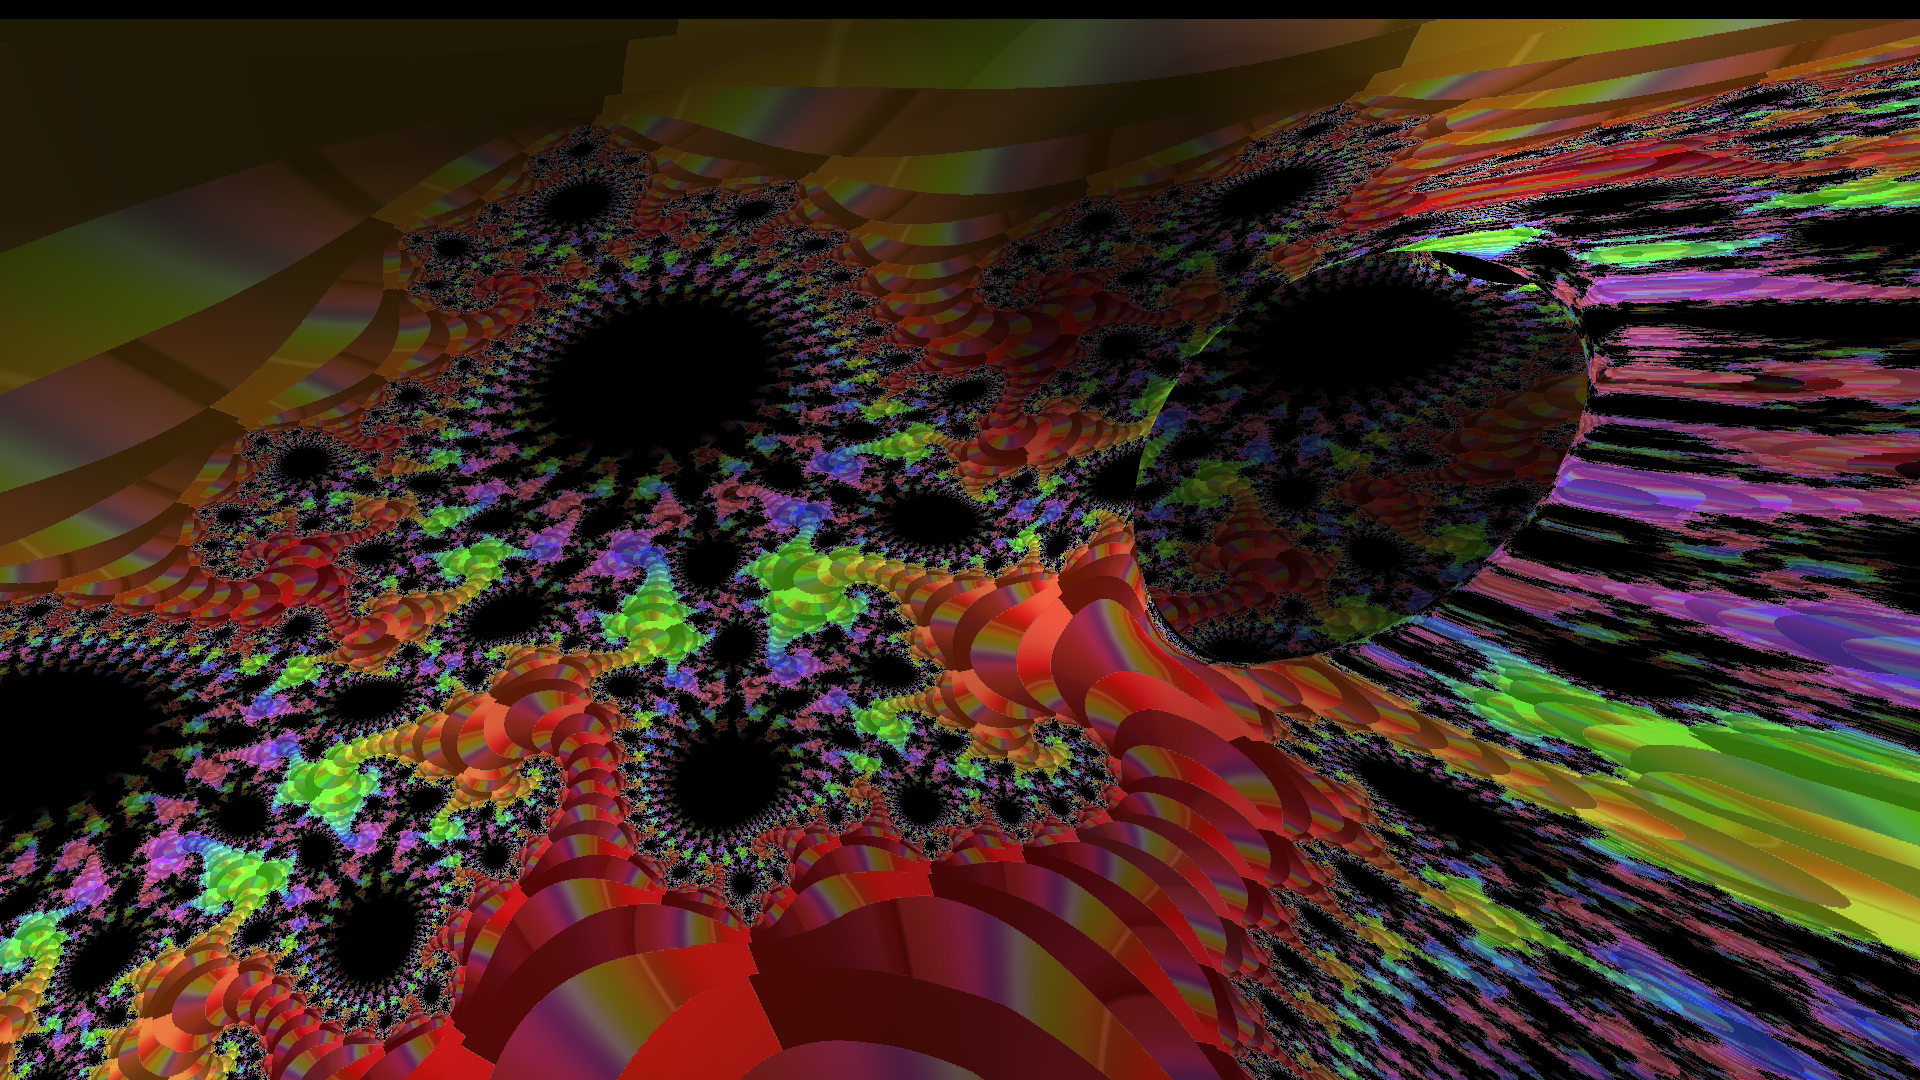
\includegraphics[scale=0.1]{o1.PNG}
}
\subfigure
{
    \label{fig:subfig1}
    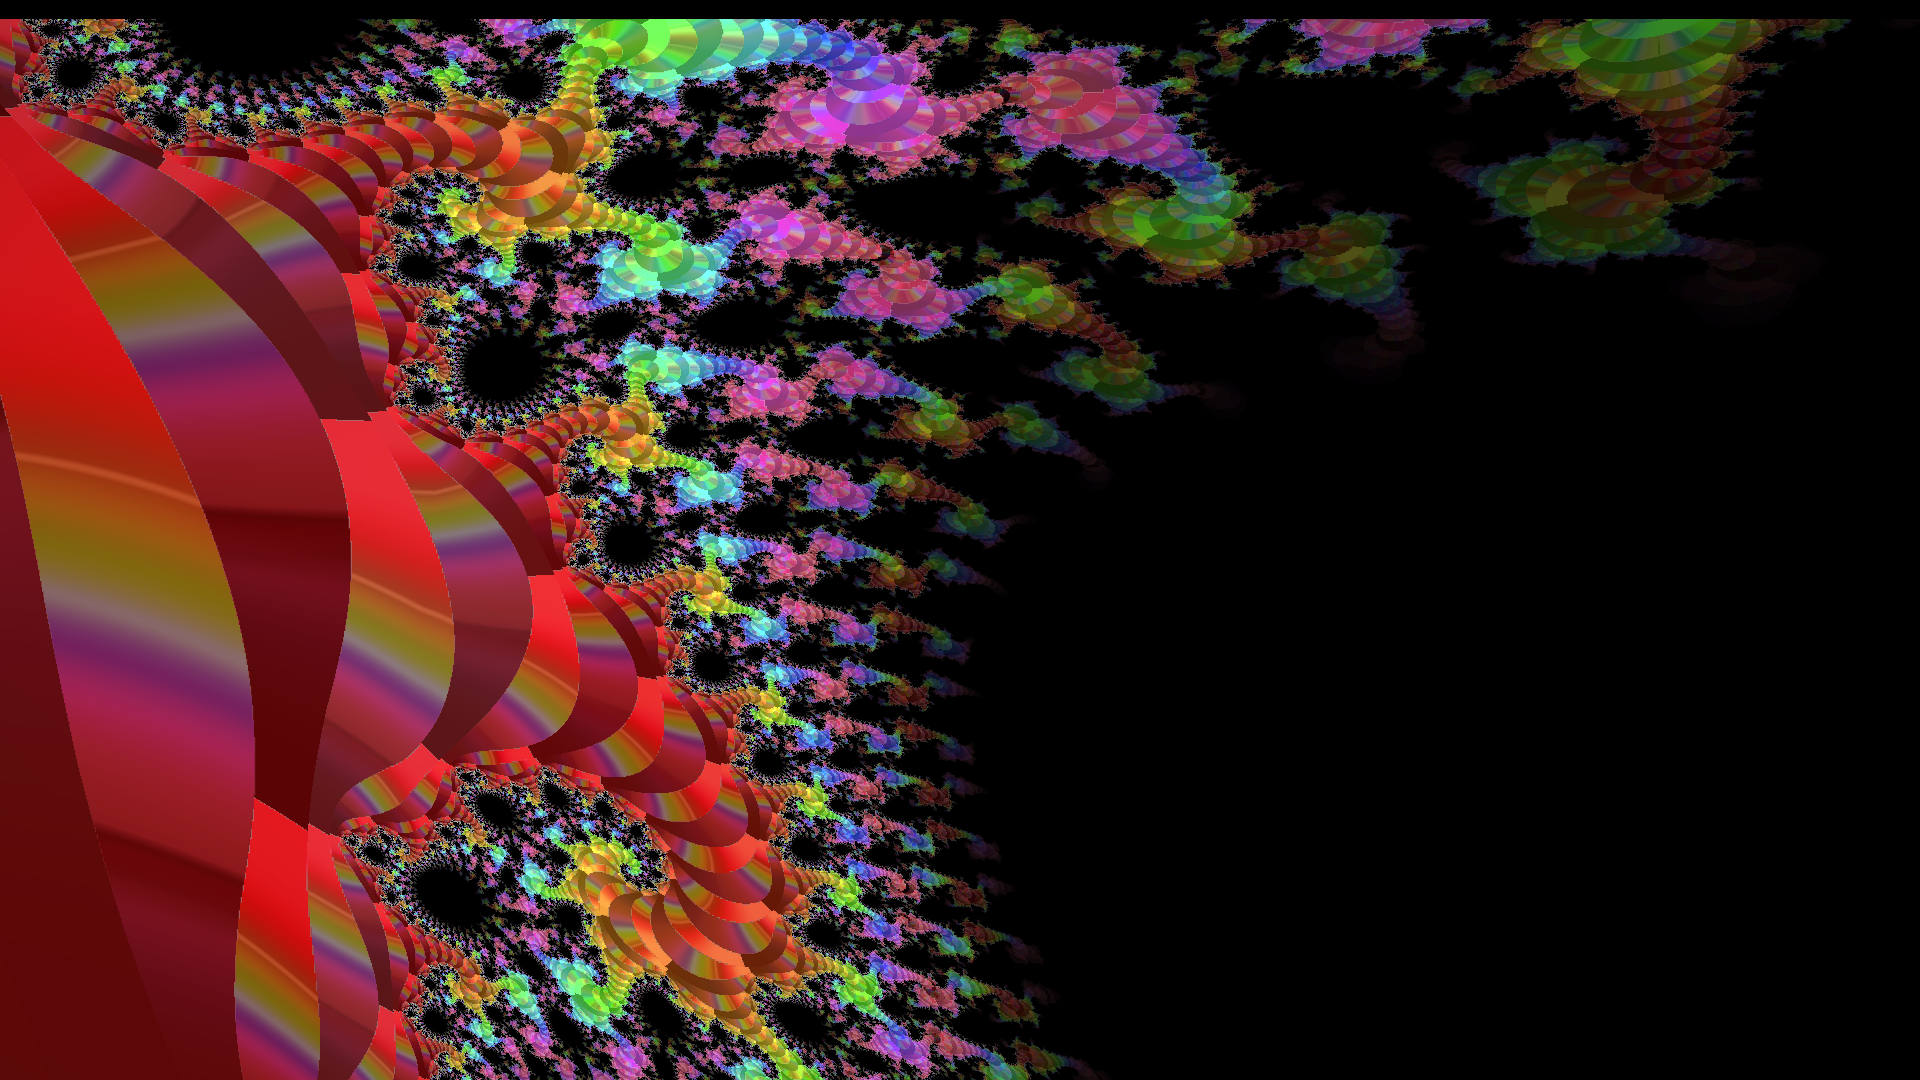
\includegraphics[scale=0.1]{o2.PNG}
}
\subfigure
{
    \label{fig:subfig1}
    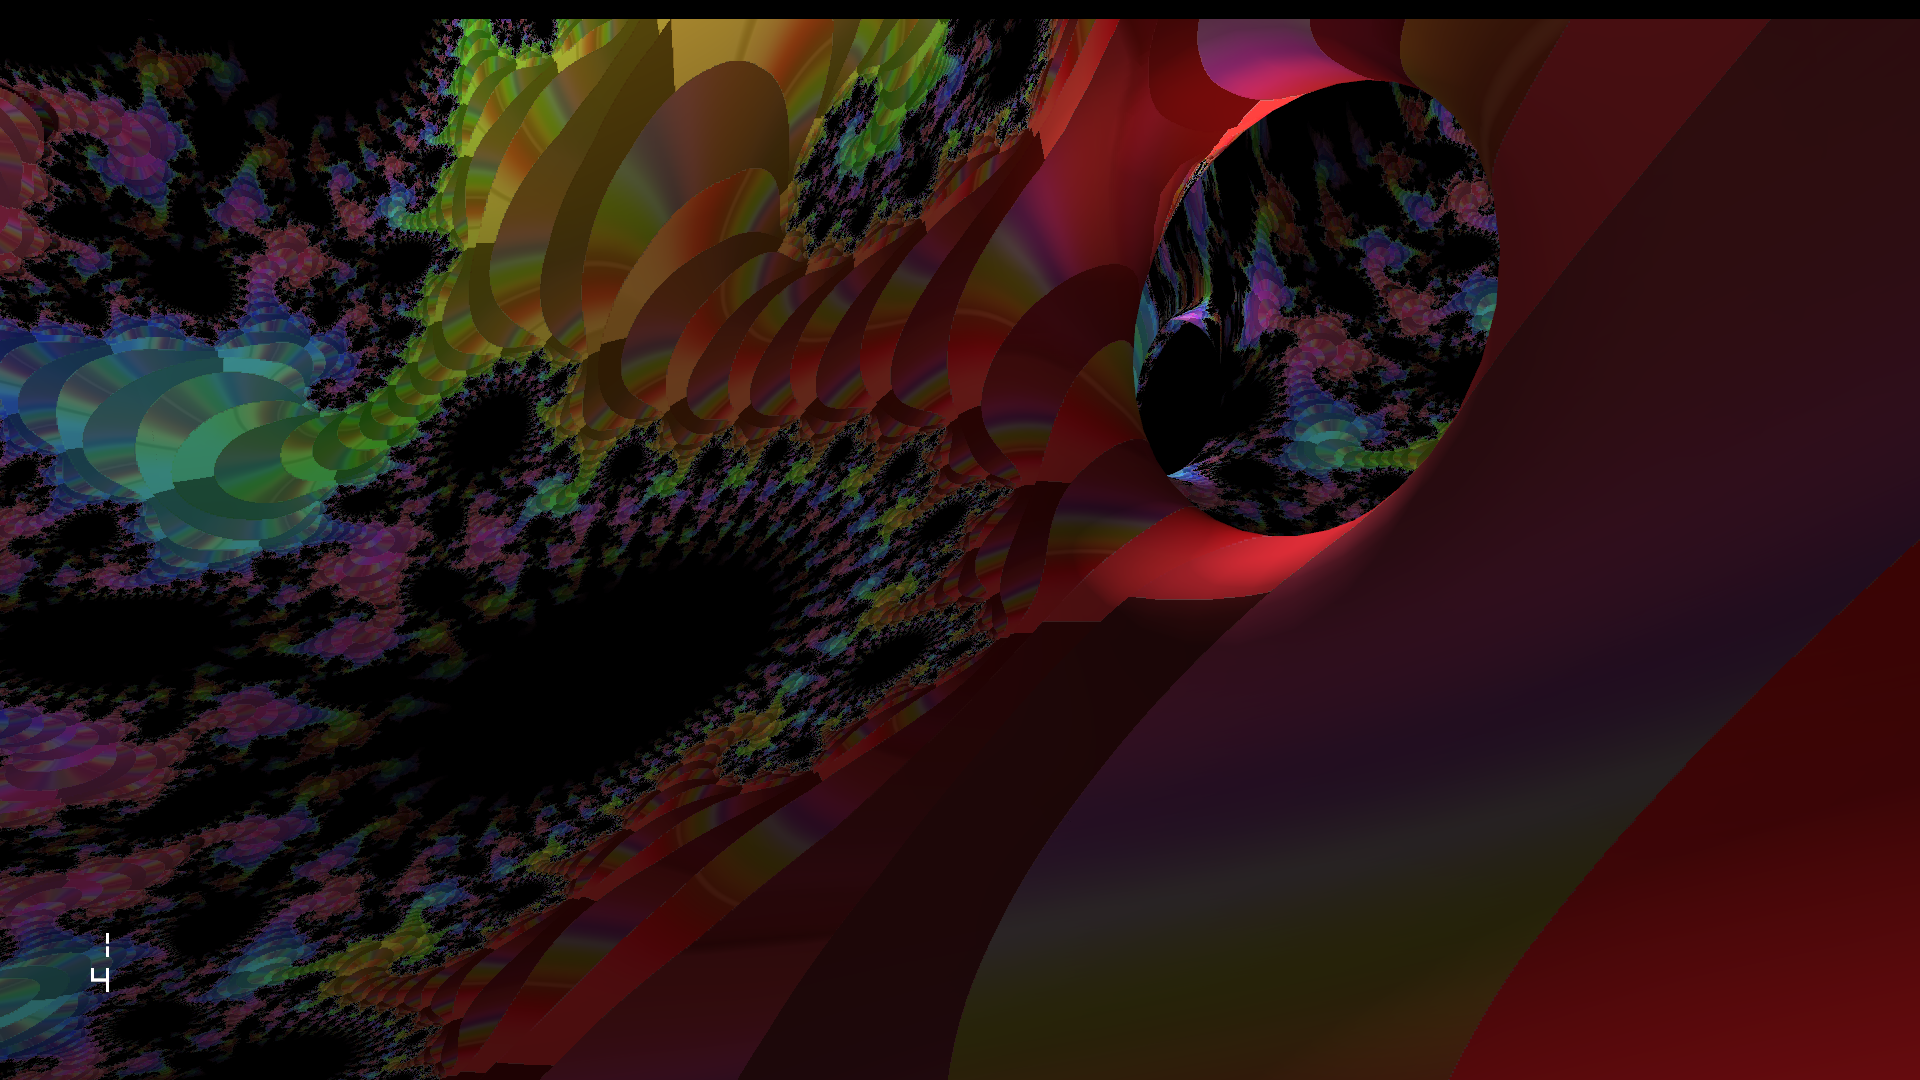
\includegraphics[scale=0.1]{o3.PNG}
}
\subfigure
{
    \label{fig:subfig1}
    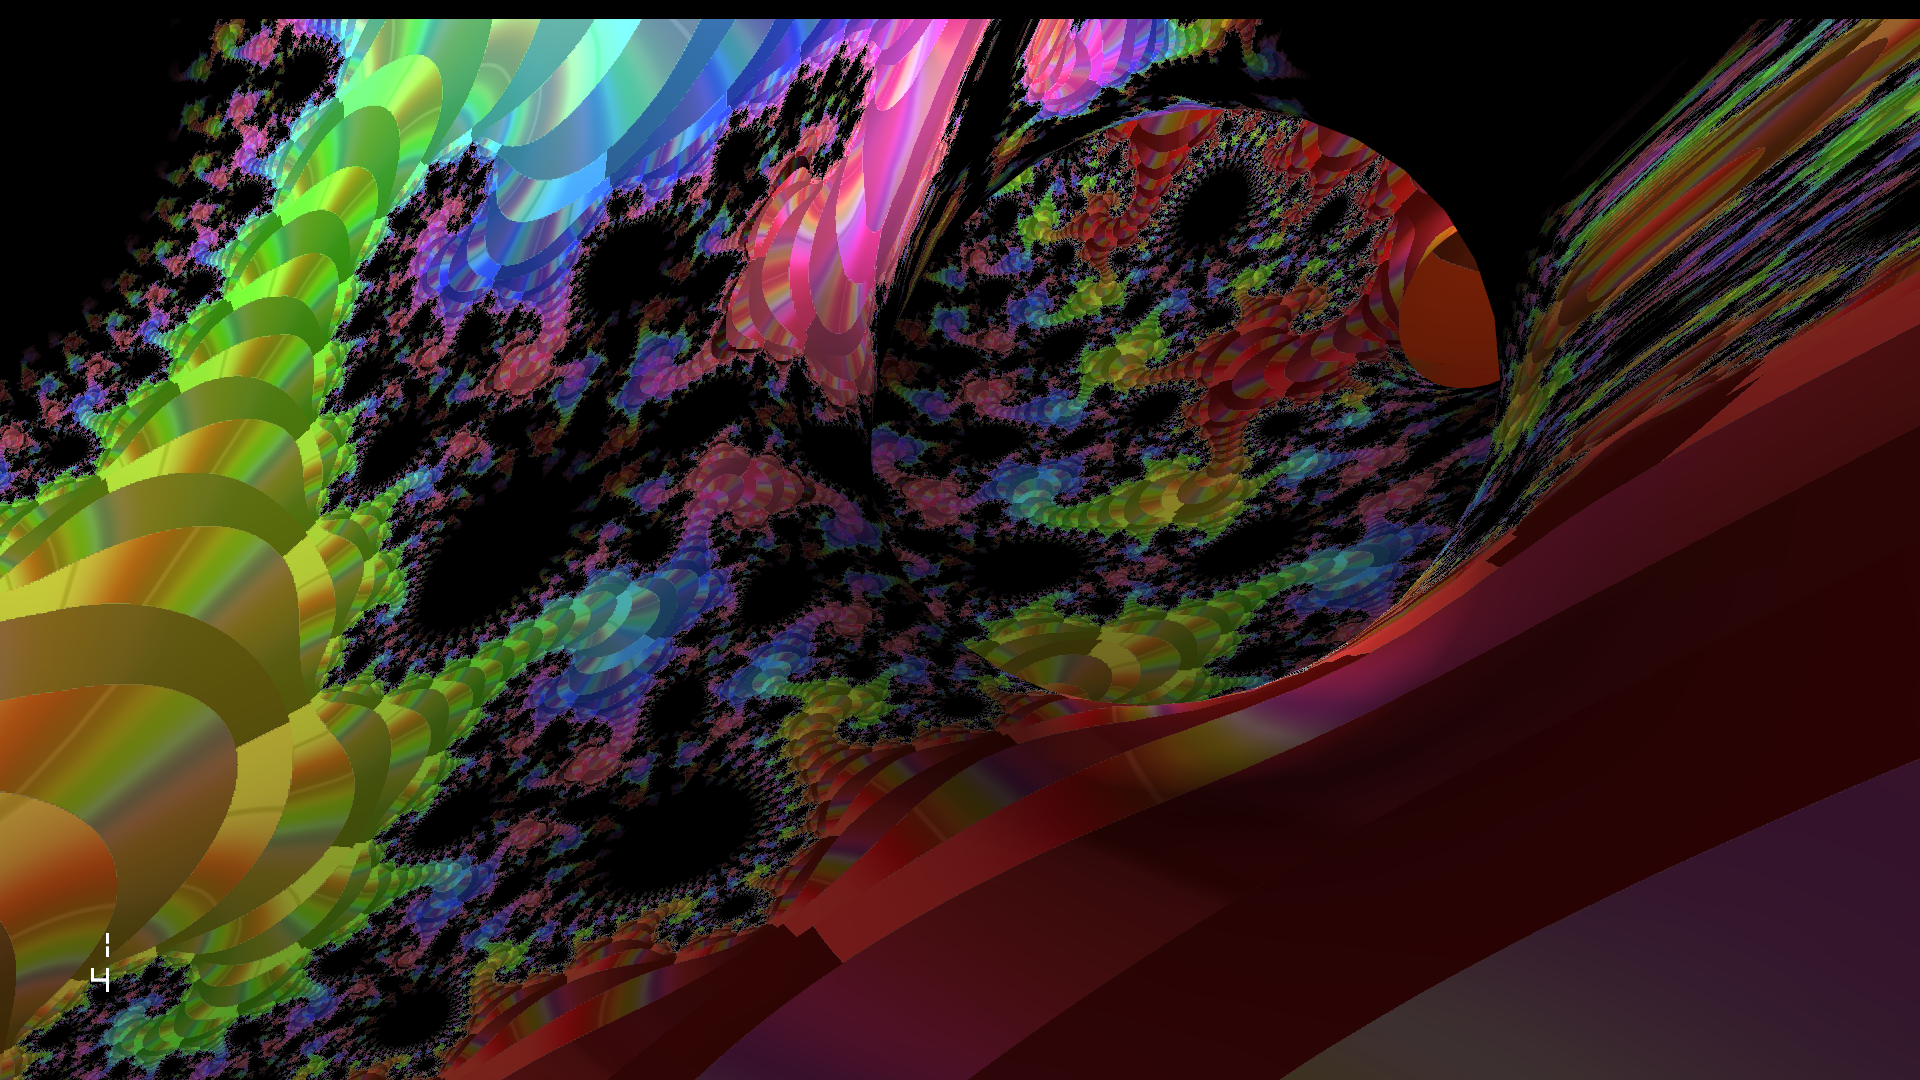
\includegraphics[scale=0.1]{o4.PNG}
}
\subfigure
{
    \label{fig:subfig1}
    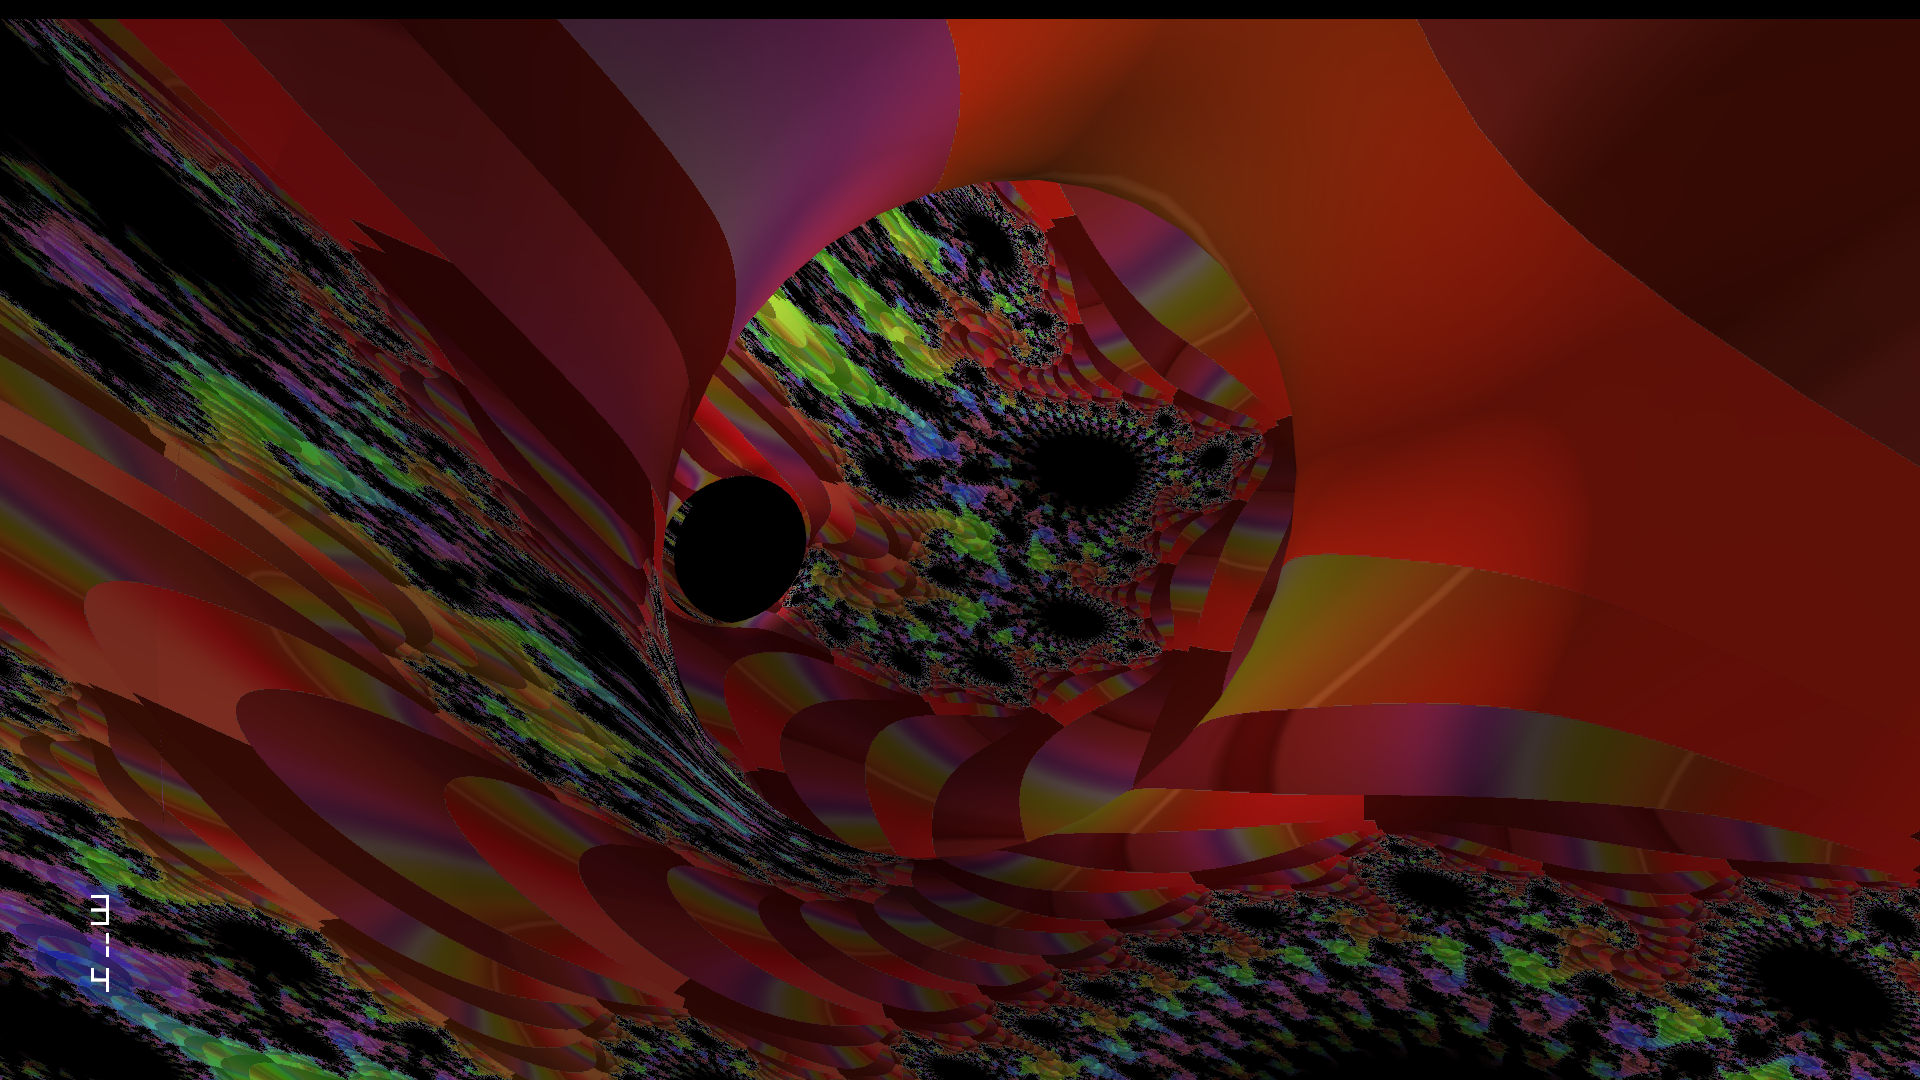
\includegraphics[scale=0.1]{o5.PNG}
}
\subfigure
{
    \label{fig:subfig1}
    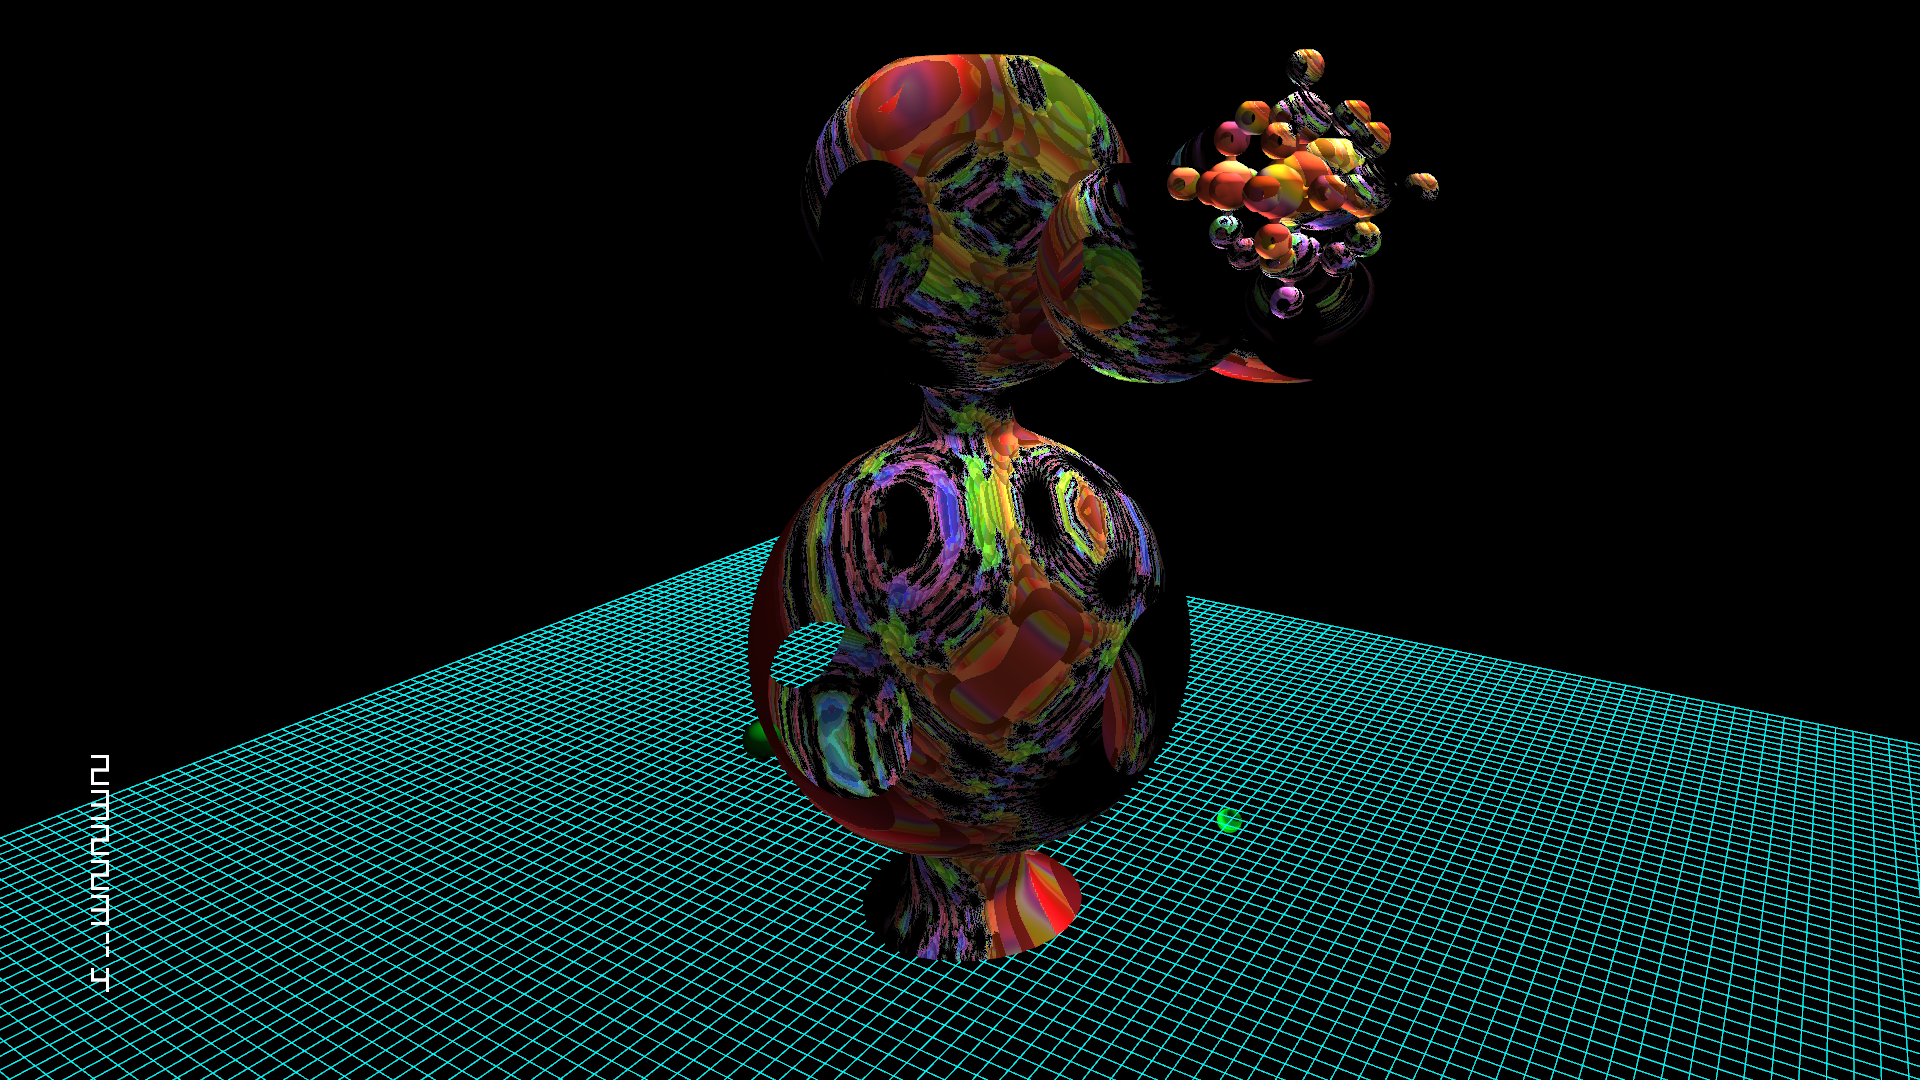
\includegraphics[scale=0.1]{o6.PNG}
}
\caption[1]{Some screenshot captures of program.}
\end{figure}



\section{Discussion}
There are some issues in this project to develop further.
\begin{description}[style=nextline]
\item[Smooth Camera Movement]
Unlike movements using a keyboard, mouse movement is calculated whenever a call-back function is called, rather than pressing a button.
Therefore it is difficult to determine when the movement of the mouse starts or stops, and so is the momentum.
Currently, we only gives interpolation to move the mouse, so it moves smoothly, but it only moves as much as the mouse did because it does not have a momentum.
Adding a term that changes the interpolation through how much the coordinate values have changed can make movement as if it were moving like an object with momentum like keyboard movement.
\item[Infinite Mandelbrot zoom]
It would be nice if infinite mandelbrot zooming is possible, but we concluded that it is impossible in our knowledge.
First, it is impossible to determine a point converges or not, because we are using an iterative algorithm.
But there is no known method for deciding convergence without doing the iteration, so the complexity of the fractal must have a limitation (the divergence determination depends on the number of loops in the iteration).
Second, the input coordinate has an accuracy problem because we use a floating point mechanism, and the floating point problem leads to poor accuracy in deep zoom depth.
Of course ther would be another level of mathematical formulation that solve all those problem, but we were not able to search that easily.
\item[Further deformation]
Current deformation on geometric fractal is limitted. The distortion stays only in each nodes, and never inherits down to further level.
This is because it is hard to keep camera's position consistent and check collision properly.
If we can do some distortion on hierarchy, then the result will be even more dramatic and complex.
\end{description}

\section{Contribution}
\begin{description}[style=nextline]
\item[Yang Junha]
Team leader, Overall design, Geometric fractal, Deformation, Texture mapping, Antialiasing, and Path tracking.
\item[Ryu Sangwoo]
3D Meshes, Camera movement, Video export and editing.
\item[Sung Haebin]
Mandelbrot set visualization, obj and Texture loading.
\end{description}

\begin{thebibliography}{1}
\bibitem{c1}E. Angel and D. Shreiner, Interactive Computer Graphics: A Top-Down Approach with Shader-Based OpenGL, 6th ed., Addison-Wesley, 2011, p.487 Section 9.8 Recursive Methods and fractals
\bibitem{c2}Graham Sellers; Richard S. Wright, Jr.; Nicholas Hanemel, OpenGL SuperBible, 7th ed., Addison-Wesley, p.683 Rendering Julia Fractals
\bibitem{c3}Rickard Englund, Rendering Methods for 3D Fractals
\bibitem{c4}Fragmentarium,\url{http://syntopia.github.io/Fragmentarium/index.html}
\end{thebibliography}

\end{document}
